\documentclass[notitlepage,a4paper,12pt,norsk]{IMFeksamen}
\usepackage{geometry}
\geometry{left=3.5cm,right=3.5cm,bottom=2cm}
\usepackage[utf8]{inputenc}
\emnekode{TMA4110}
\emnenavn{Matematikk 3}
\eksamensdato{4. desember 2018}
\eksamenstid{09:00–13:00}
\fagligkontaktinfo{Øystein Skartsæterhagen}{}
\hjelpemiddel{Ingen trykte eller håndskrevne hjelpemidler tillatt.
 Bestemt, enkel kalkulator tillatt.
 (Casio fx-82ES PLUS, Casio fx-82EX,
  Citizen SR-270X, Citizen SR-270X College,
  Hewlett Packard HP30S)}
\runninghead{TMA4110 Matematikk 3 -- Eksamen høsten 2018 -- Løsning}
\usepackage[T1]{fontenc}
\usepackage{lmodern,amsmath,amssymb,amsfonts}
\usepackage{mathrsfs}
\usepackage{systeme}
\usepackage{pgfornament}
\usepackage{tikz,pgfplots}

\newcommand{\N}{\mathbb{N}}
\newcommand{\Z}{\mathbb{Z}}
\newcommand{\Q}{\mathbb{Q}}
\newcommand{\R}{\mathbb{R}}
\newcommand{\C}{\mathbb{C}}

\newcommand{\M}{\mathcal{M}} % vektorrom av matriser
\newcommand{\Cf}{\mathcal{C}} % vektorrom av kontinuerlige funksjoner
\renewcommand{\P}{\mathcal{P}} % vektorrom av polynomer
\newcommand{\B}{\mathscr{B}} % basis

\renewcommand{\Im}{\operatorname{Im}}
\renewcommand{\Re}{\operatorname{Re}}

\newcommand{\abs}[1]{|#1|}
\newcommand{\intersect}{\cap}
\newcommand{\union}{\cup}
\newcommand{\fcomp}{\circ}
\newcommand{\iso}{\cong}

\newcommand{\roweq}{\sim}
\DeclareMathOperator{\Sp}{Sp}
\DeclareMathOperator{\Null}{Null}
\DeclareMathOperator{\Col}{Col}
\DeclareMathOperator{\Row}{Row}
\DeclareMathOperator{\rank}{rank}
\DeclareMathOperator{\im}{im}
\DeclareMathOperator{\id}{id}
\DeclareMathOperator{\Hom}{Hom}
\newcommand{\tr}{^\top}
\newcommand{\koord}[2]{[\,{#1}\,]_{#2}} % koordinater mhp basis

\newcommand{\V}[1]{\mathbf{#1}}
\newcommand{\vv}[2]{\begin{bmatrix} #1 \\ #2 \end{bmatrix}}
\newcommand{\vvS}[2]{\left[ \begin{smallmatrix} #1 \\ #2 \end{smallmatrix} \right]}
\newcommand{\vvv}[3]{\begin{bmatrix} #1 \\ #2 \\ #3 \end{bmatrix}}
\newcommand{\vvvv}[4]{\begin{bmatrix} #1 \\ #2 \\ #3 \\ #4 \end{bmatrix}}
\newcommand{\vvvvv}[5]{\begin{bmatrix} #1 \\ #2 \\ #3 \\ #4 \\ #5 \end{bmatrix}}
\newcommand{\vn}[2]{\vvvv{#1_1}{#1_2}{\vdots}{#1_#2}}

\newcommand{\e}{\V{e}}
\renewcommand{\u}{\V{u}}
\renewcommand{\v}{\V{v}}
\newcommand{\w}{\V{w}}
\renewcommand{\a}{\V{a}}
\renewcommand{\b}{\V{b}}
\renewcommand{\c}{\V{c}}
\newcommand{\x}{\V{x}}
\newcommand{\0}{\V{0}}

\newenvironment{amatrix}[1]{% "augmented matrix"
  \left[\begin{array}{*{#1}{c}|c}
}{%
  \end{array}\right]
}

\newcommand{\oppgslutt}{
\begin{center}
\pgfornament[width=6cm]{88}
\end{center}
}
\newenvironment{losning}{\begin{oppgave}}{\oppgslutt\end{oppgave}}


\begin{document}


\begin{center}
\textbf{\large Løsningsforslag} \\[3pt]
\pgfornament[width=6cm]{88}
\end{center}
\vspace{-10pt}


\begin{losning}
Vi setter opp totalmatrisen og gausseliminerer:
\begin{align*}
\begin{amatrix}{3}
1 & -1 & 2 & 28 \\
-2 & 5 & -4 & -20 \\
-1 & 1 & -1 & -10
\end{amatrix}
&\roweq
\begin{amatrix}{3}
1 & -1 & 2 & 28 \\
0 & 3 & 0 & 36 \\
0 & 0 & 1 & 18
\end{amatrix}
\roweq
\begin{amatrix}{3}
1 & -1 & 2 & 28 \\
0 & 1 & 0 & 12 \\
0 & 0 & 1 & 18
\end{amatrix}
\\
&\roweq
\begin{amatrix}{3}
1 & 0 & 0 & 4 \\
0 & 1 & 0 & 12 \\
0 & 0 & 1 & 18
\end{amatrix}
\end{align*}
Den siste matrisen her er på redusert trappeform,
og vi får entydig løsning:
\[
\systeme*{
x = 4,
y = 12,
z = 18
}
\]
(Hvorfor valgte vi akkurat disse tallene?
Fordi eksamenen var den $x$-te dagen i den $y$-te måneden i år
totusenog$z$.)
\end{losning}


\begin{losning}
Vi skal finne ut to ting:
Om vektorene $\v_1$, $\v_2$ og~$\v_3$ er lineært uavhengige,
og om $\b$ er en lineærkombinasjon av $\v_1$, $\v_2$ og~$\v_3$.
Vi kan besvare begge spørsmålene ved å gausseliminere totalmatrisen
$
\begin{amatrix}{3}
\v_1 & \v_2 & \v_3 & \b
\end{amatrix}
$.
Vi gjør dette:
\begin{align*}
\begin{amatrix}{3}
3 & -2 & 1 & 4 \\
-3 & 2 & -1 & -9 \\
-6 & 4 & -8 & 3
\end{amatrix}
&
\roweq
\begin{amatrix}{3}
3 & -2 & 1 & 4 \\
0 & 0 & 0 & -5 \\
0 & 0 & -6 & 11
\end{amatrix}
\roweq
\begin{amatrix}{3}
3 & -2 & 1 & 4 \\
0 & 0 & -6 & 11 \\
0 & 0 & 0 & -5
\end{amatrix}
\end{align*}
Vi ser at vektorene $\v_1$, $\v_2$ og~$\v_3$ ikke er lineært uavhengige,
siden det ikke er noe pivotelement i den andre kolonnen.
Vektoren $\b$ er ikke en lineærkombinasjon av $\v_1$, $\v_2$ og~$\v_3$,
siden vi får den selvmotsigende likningen $0 = -5$ fra siste rad.

Begge spørsmålene i oppgaven har altså svaret \emph{nei}.
\end{losning}


\begin{minipage}[t]{.5\textwidth}
\begin{oppgave}
Likningssystemet kan skrives på matriseform slik:
\[
\begin{bmatrix}
y_1  \\
y_2
\end{bmatrix}'
=
\begin{bmatrix}
7 & -2  \\
2 & 2 
\end{bmatrix}
\begin{bmatrix}
y_1  \\
y_2 
\end{bmatrix}
\]
Egenverdiene til matrisen er $2$ og~$1$,
med egenvektorer henholdsvis
$\vvS{2}{1}$ og~$\vvS{1}{2}$.
Den generelle løsningen av systemet er
\[
\mathbf y(t)=
c_1e^{2t}
\begin{bmatrix}
2  \\
1 
\end{bmatrix}
+ 
c_2e^{t}
\begin{bmatrix}
1  \\
2 
\end{bmatrix}.
\]
\end{oppgave}
\end{minipage}
\hfill
\begin{minipage}[t]{.4\textwidth}
\begin{center}
%\hbox{}\\
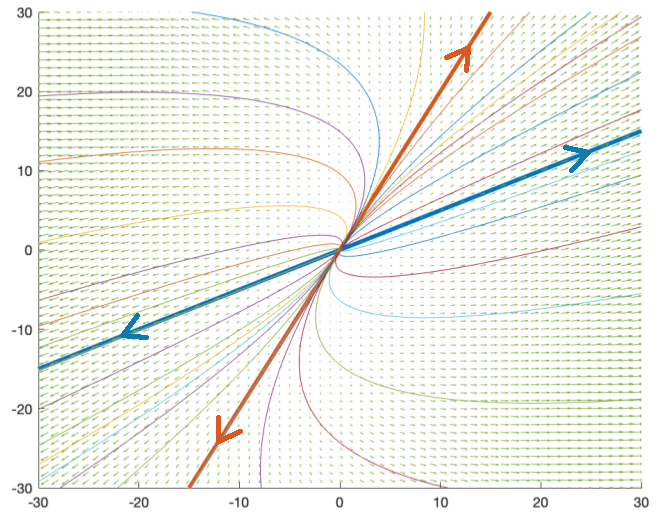
\includegraphics[scale=.35]{fasediagram}\\
Fasediagram
\end{center}
\end{minipage}
\vspace{-20pt}
\oppgslutt


\begin{losning}
Vi finner først andregradspolynomet
$p(x)=ax^2+bx+c$
som passer eksakt til de tre punktene.
Da må vi ha
\[
p(0) = -1,\quad
p(1) = 1\quad
\text{og}\quad
p(2) = 7,
\]
så vi kan sette opp likningssystemet
\[
\systeme{
c=-1,
a+b+c=1,
4a+2b+c=7
}
\]
for koeffisientene i~$p$.
Dette systemet har én løsning: $a=2$, $b=0$ og $c=-1$.
Polynomet blir altså $p(x) = 2x^2 - 1$. 

Nå skal vi finne det førsteordens polynomet
$q(x) = dx + e$
som passer best til punktene.
Hvis $q$ skulle passet eksakt til punktene, ville vi hatt
\[
q(0) = -1,\quad
q(1) = 1\quad
\text{og}\quad
q(2) = 7,
\]
som gir følgende likningssystem for koeffisientene:
\[
\systeme{
e=-1,
d+e=1,
2d+e=7
}
\]
Skrevet på matriseform ser det slik ut:
\[
\begin{bmatrix}
0 & 1  \\
1 & 1  \\
2 & 1 
\end{bmatrix}
\begin{bmatrix}
a  \\
b 
\end{bmatrix}
=
\begin{bmatrix}
-1  \\
1  \\
7
\end{bmatrix}.
\]
Vi finner den beste tilnærmingen til en løsning ved å bruke
minste kvadraters metode.
Da må vi gange begge sider av likningen med den transponerte
\[
\begin{bmatrix}
0 & 1 & 2 \\
1 & 1 & 1
\end{bmatrix}
\]
av koeffisientmatrisen.  Det gir oss likningssystemet
\[
\begin{bmatrix}
5 & 3  \\
3 & 3 
\end{bmatrix}
\begin{bmatrix}
d  \\
e 
\end{bmatrix}
=
\begin{bmatrix}
15  \\
7
\end{bmatrix},
\]
som har løsning $d=4$ og $e=1$. Polynomet er $q(x) = 4x + 1$.
% TODO: Skisse?
\begin{center}
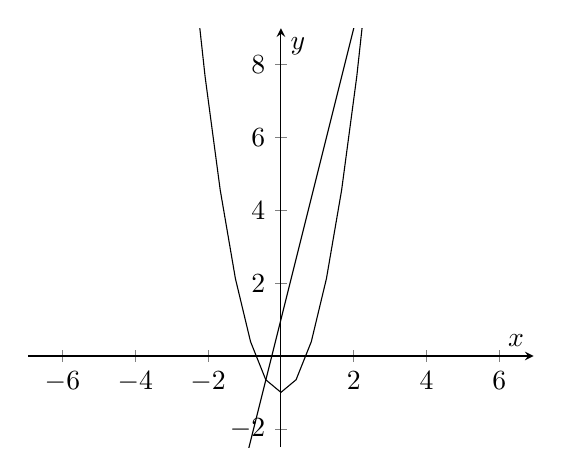
\begin{tikzpicture}[baseline]
\begin{axis}[
axis y line=center,
axis x line=middle,
axis equal,
%grid=both,
xmax=5,xmin=-5,
ymin=-2.5,ymax=9,
xlabel=$x$,ylabel=$y$,
%xtick={-5,...,5},
%ytick={-1,...,8},
width=8cm,
anchor=center,
]
\addplot[black] {2*x^2 - 1} ;
\addplot[black] {4*x + 1} ;
\end{axis}
\end{tikzpicture}
\end{center}
\end{losning}


\begin{losning}
Vi skal finne alle $2 \times 2$-matriser~$X$ som er løsninger av likningen
$AX = XA$, der
\[
A =
\begin{bmatrix}
 9 & -3 \\
-3 &  2
\end{bmatrix}
\]
La oss kalle de fire tallene i matrisen~$X$ for $x_1$, $x_2$, $x_3$ og~$x_4$:
\[
X =
\begin{bmatrix}
x_1 & x_2 \\
x_3 & x_4
\end{bmatrix}
\]
Vi skriver opp hvordan matrisene $AX$ og~$XA$ ser ut:
\begin{align*}
AX &=
\begin{bmatrix}
 9 & -3 \\
-3 &  2
\end{bmatrix}
\begin{bmatrix}
x_1 & x_2 \\
x_3 & x_4
\end{bmatrix}
=
\begin{bmatrix}
 9 x_1 - 3 x_3  &   9 x_2 - 3 x_4  \\
-3 x_1 + 2 x_3  &  -3 x_2 + 2 x_4
\end{bmatrix}
\\
XA &=
\begin{bmatrix}
x_1 & x_2 \\
x_3 & x_4
\end{bmatrix}
\begin{bmatrix}
 9 & -3 \\
-3 &  2
\end{bmatrix}
=
\begin{bmatrix}
9 x_1 - 3 x_2  &  -3 x_1 + 2 x_2  \\
9 x_3 - 3 x_4  &  -3 x_3 + 2 x_4
\end{bmatrix}
\end{align*}
Likningen $AX = XA$ er altså ekvivalent med dette systemet av fire
likninger:
\[
\left\{
\begin{aligned}
 9 x_1 - 3 x_3 &=  9 x_1 - 3 x_2 \\
 9 x_2 - 3 x_4 &= -3 x_1 + 2 x_2 \\
-3 x_1 + 2 x_3 &=  9 x_3 - 3 x_4 \\
-3 x_2 + 2 x_4 &= -3 x_3 + 2 x_4
\end{aligned}
\right.
\]
Vi flytter alt over til venstresiden i hver likning og forenkler:
\[
\systeme*{
3x_2 - 3x_3 = 0,
3x_1 + 7x_2 - 3x_4 = 0,
-3x_1 - 7x_3 + 3x_4 = 0,
-3x_2 + 3x_3 = 0
}
\]
Dette er et vanlig lineært likningssystem,
så vi kan sette opp koeffisientmatrisen og gausseliminere:
\[
\begin{bmatrix}
 0 &  3 & -3 &  0 \\
 3 &  7 &  0 & -3 \\
-3 &  0 & -7 &  3 \\
 0 & -3 &  3 &  0
\end{bmatrix}
\roweq
\begin{bmatrix}
1 & 0 & 7/3 & -1 \\
0 & 1 &  -1 &  0 \\
0 & 0 &   0 &  0 \\
0 & 0 &   0 &  0
\end{bmatrix}
\]
Vi får to frie variabler, og den generelle løsningen blir
\[
\left.
\begin{aligned}
x_1 &= -\frac{7}{3} s + t \\
x_2 &= s \\
x_3 &= s \\
x_4 &= t
\end{aligned}
\;\right\}
\qquad
\text{der $s$ og~$t$ er vilkårlige tall.}
\]
Dette betyr at alle løsninger av likningen $AX = XA$ er gitt ved
\[
X =
\begin{bmatrix}
-7/3 & 1 \\
 1   & 0
\end{bmatrix}
s
+
\begin{bmatrix}
1 & 0 \\
0 & 1
\end{bmatrix}
t
\qquad
\text{der $s$ og~$t$ er vilkårlige tall.}
\]
\end{losning}


\begin{losning}
La
$U = \Sp \{ \v_1, \v_2, \v_3, \v_4 \}$
være rommet vi skal finne en ortogonal basis for.
Det er lett å se at $\v_4$ er en lineærkombinasjon av
de andre vektorene, siden $\v_4 = \v_2 + \v_3$.
Det er heller ikke vanskelig å se at vektorene
$\v_1$, $\v_2$ og~$\v_3$
er lineært uavhengige,
slik at $(\v_1, \v_2, \v_3)$ er en basis for~$U$.

Vi ortogonaliserer basisen med Gram--Schmidt-metoden:
\begin{align*}
\u_1 &= \v_1 \\
\u_2 &= \v_2 - \frac{\u_1\tr \v_2}{\u_1\tr \u_1} \u_1 = \v_2 - 0 \cdot \u_1 = \v_2 \\
\u_3 &= \v_3 - \frac{\u_1\tr \v_3}{\u_1\tr \u_1} \u_1 - \frac{\u_2\tr \v_3}{\u_2\tr \u_2} \u_2
      = \vvvv{1}{1}{1}{0} - \frac{4}{6} \vvvv{2}{1}{1}{0} - \frac{-1}{6} \vvvv{1}{0}{-2}{1}
      = \vvvv{-1/6}{2/6}{0}{1/6}
\end{align*}
Nå er $(\u_1, \u_2, \u_3)$ en ortogonal basis for~$U$.
Siden lengden av hver vektor ikke spiller noen rolle,
kan vi alternativt erstatte $\u_3$ med $6 \cdot \u_3$ for å få penere tall;
da ender vi opp med følgende ortogonale basis:
\[
\left(
\vvvv{2}{1}{1}{0},\ %
\vvvv{1}{0}{-2}{1},\ %
\vvvv{-1}{2}{0}{1}
\right)
\]
\end{losning}


\begin{losning}
Her er to forskjellige forslag til løsning:

\emph{Løsning~1,
der vi husker at diagonalisering gjør det enkelt
å beregne potenser av matriser.}
\ %
Hvis vi klarer å diagonalisere matrisen~$R$,
så blir det enklere å regne ut~$R^{\,42}$.
Vi starter derfor med å finne egenverdier og egenvektorer.
Det karakteristiske polynomet til~$R$ er
\[
\begin{vmatrix}
        1/2 - \lambda & \sqrt{3}/2           \\
-\sqrt{3}/2           &        1/2 - \lambda
\end{vmatrix}
= \left( \frac{1}{2} - \lambda \right)^2 + \frac{3}{4}
= \lambda^2 - \lambda + 1,
\]
og vi får egenverdiene
\[
\lambda_1 = \frac{1}{2} + \frac{\sqrt{3}}{2}
\qquad\text{og}\qquad
\lambda_2 = \frac{1}{2} - \frac{\sqrt{3}}{2}.
\]
Vi regner ut, på vanlig måte, at vektorene
\[
\v_1 = \vv{1}{i}
\qquad\text{og}\qquad
\v_2 = \vv{1}{-i}
\]
er egenvektorer som hører til henholdsvis $\lambda_1$ og~$\lambda_2$.
Vi får altså en diagonalisering
\[
R = VDV^{-1}
\]
av matrisen~$R$, der matrisene $V$ og~$D$ er gitt ved:
\[
V =
\begin{bmatrix}
1 &  1 \\
i & -i
\end{bmatrix}
\qquad\qquad
D =
\begin{bmatrix}
\lambda_1 & 0         \\
0         & \lambda_2
\end{bmatrix}
\]
Nå vil vi regne ut $D^{\,42}$.
Da er det en fordel å skrive de komplekse egenverdiene
$\lambda_1$ og~$\lambda_2$ på polarform:
\begin{align*}
\lambda_1 &= e^{\frac{\pi}{3} i} \\
\lambda_2 &= e^{-\frac{\pi}{3} i}
\end{align*}
Dette gjør at vi får
\begin{align*}
\lambda_1^{42} &= e^{42 \cdot \frac{\pi}{3} i} = e^{21 \cdot 2\pi i} = 1 \\
\lambda_2^{42} &= e^{42 \cdot (-\frac{\pi}{3} i)} = e^{(-21) \cdot 2\pi i} = 1,
\end{align*}
slik at
\[
D^{\,42} =
\begin{bmatrix}
\lambda_1^{42} & 0              \\
0              & \lambda_2^{42}
\end{bmatrix}
=
\begin{bmatrix}
1 & 0 \\
0 & 1
\end{bmatrix}
= I_2.
\]
Dette betyr at vi har:
\[
R^{\,42} = V D^{\,42} V^{-1} = V I_2 V^{-1} = V V^{-1} = I_2
\]

\emph{Løsning~2,
der vi ikke husker de der diagonaliseringsgreiene,
men er litt lure isteden.}
\ %
Siden
$\cos \frac{\pi}{3}=\frac{1}{2}$
og
$\sin \frac{\pi}{3}=\frac{\sqrt{3}}{2}$,
ser vi at matrisen~$R$ også kan skrives slik:
\[
R =
\begin{bmatrix}
 \cos \frac{\pi}{3} & \sin \frac{\pi}{3} \\[4pt]
-\sin \frac{\pi}{3} & \cos \frac{\pi}{3}
\end{bmatrix}
\]
Dette er en rotasjonsmatrise som roterer vektorer
$\frac{\pi}{3}$
radianer med klokken.
Å anvende denne matrisen seks ganger gir en full rotasjon,
slik at $R^6 \v = \v$ for alle vektorer~$\v$.
Det vil si at $R^{\,6}$ er identitetsmatrisen~$I_2$,
og vi får
\[
R^{\,42} = \big( R^{\,6} \big)^7 = I_2^7 = I_2.
\]
\end{losning}


\begin{losning}
Vi følger standard metode for å finne kolonne- og nullrommet til $A$,
så vi begynner med å gausseliminere:
\[
A =
\begin{bmatrix}
2 & i & 5-3i\\
4 & 2i & 10+2i\\
2i & -1 & 4+6i
\end{bmatrix}
\roweq
\begin{bmatrix}
2 & i & 5-3i\\
0 & 0 & 8i\\
0 & 0 & 1+i
\end{bmatrix}
\roweq
\begin{bmatrix}
2 & i & 5-3i\\
0 & 0 & 8i\\
0 & 0 & 0
\end{bmatrix}
\roweq
\begin{bmatrix}
2 & i & 0 \\
0 & 0 & 1 \\
0 & 0 & 0
\end{bmatrix}
\]
Pivotelement i første og tredje kolonne viser at
\[
\left( \vvv{2}{4}{2i}, \vvv{5-3i}{10+2i}{4+6i} \right)
\]
er en basis for $\Col A$.

Nullrommet består av alle løsninger av likningen $A \x = \0$.
Gausseliminasjonen over gir at denne likningen kan skrives som
følgende system:
\[
\systeme*{
2x_1 + ix_2 = 0,
x_3 = 0
}
\]
Den generelle løsningen blir
\[
\x = \vvv{-i/2}{1}{0} t
\qquad\text{der $t$ er et vilkårlig komplekst tall.}
\]
Dermed er
\[
\left( \vvv{-i/2}{1}{0} \right)
\]
en basis for $\Null A$.
% Dette gir $x_3=0$ slik at
% \[
% 2x_1+ix_2=0.
% \]
% Det er én fri variabel. Vi kan for eksempel bruke $x_2$ til å parametrisere nullrommet: $x_2=t$. Dette gir 
% \[
% \Null A=\{t\vvv{-\frac{i}{2}}{1}{0}|\;\; t \in \mathbb{C}\}.
% \]
% Alle $t\neq 0$ gir et valg av basis. Vi kan for eksempel ta $t=1$ for å se at \[
% \Big(\vvv{-\frac{i}{2}}{1}{0}\Big)
% \]
%  er en basis for $\Null A$. 
 
Til slutt skal vi finne alle vektorer $\v$ i~$\C^3$ slik at $A\v=\0$ og $\|\v\|=1$.
At $A\v=\0$ er det samme som at $\v$ ligger i nullrommet til $A$,
og vi har allerede funnet en basis for nullrommet.
For å finne vektorer i nullrommet som har lengde~$1$, normaliserer vi basisvektoren vår.
Lengden av basisvektoren vi fant er:
\[
\left\| \vvv{-i/2}{1}{0} \right\|
= \sqrt{ \left( \frac{i}{2} \right) \left( -\frac{i}{2} \right) + 1 }
= \frac{\sqrt{5}}{2}
\]
Det vil si at vektoren
\[
\u = \vvv{-i/\sqrt{5}}{2/\sqrt{5}}{0}
\]
er en vektor med lengde~$1$ som utspenner $\Null A$.
Alle vektorer i nullrommet er på formen $t \u$ der $t$ er et komplekst tall,
og lengden av en slik vektor blir
\[
\| t \u \| = |t| \| u \| = |t|,
\]
slik at lengden er~$1$ hvis og bare hvis tallet $t$ har absoluttverdi~$1$.
De komplekse tallene som har absoluttverdi~$1$ er alle tallene på formen
$e^{i\theta}$ for en vilkårlig vinkel~$\theta$.
Alle vektorene $\v$ som er slik at $A\v = \0$ og $\| \v \| = 1$ blir altså:
\[
\v = \vvv{-i/\sqrt{5}}{2/\sqrt{5}}{0} e^{i\theta}
\qquad
\text{for en vilkårlig $\theta$ i intervallet $[0,2\pi)$.}
\]
% Vi fant en eksplisitt beskrivelse av $\Null A$:
%  vektorene er på formen $t\vvv{-\frac{i}{2}}{1}{0}$ hvor $t$ er et komplekst tall. Det siste kravet gir likningen
%  \begin{align*}
%  1&=\|t\vvv{-\frac{i}{2}}{1}{0}\|=\sqrt{(t\vvv{-\frac{i}{2}}{1}{0})^{\ast} (t\vvv{-\frac{i}{2}}{1}{0}) }\\ &=\sqrt{|-\frac{i}{2}t|^2+|t|^2}=\sqrt{\frac{1}{4}|t|^2+|t|^2}\\
%  &=|t|\sqrt{\frac{1}{4}+1}=|t|\sqrt{\frac{5}{4}}\\
%  &=|t|\frac{\sqrt{5}}{2}.
%  \end{align*}
%  Løsningen er alle $t\in \mathbb{C}$ slik at $|t|=\frac{2}{\sqrt{5}}$. For å få en mer geometrisk beskrivelse kan man ekvivalent skrive
%  \[
%  t=|t|e^{i\theta}=\frac{2}{\sqrt{5}}e^{i\theta}
%  \]
%  hvor $\theta \in [0,2\pi)$ -- en sirkel i det komplekse planet med radius $\frac{2}{\sqrt{5}}$. Dermed blir en mulig parametrisering av svaret
%  \[
%  \{\vvv{-\frac{i}{\sqrt{5}}}{\frac{2}{\sqrt{5}}}{0}e^{i\theta}|\;\; \theta\in [0,2\pi)\}.
%  \]
\end{losning}


\begin{losning}
Vi skal vise at funksjonen~$T$ er en lineærtransformasjon.
Vi kan først legge merke til at transponeringsoperasjonen er lineær,
altså at
\[
(M + N)\tr = M\tr + N\tr
\qquad
\text{og}
\qquad
(kM)\tr = k (M\tr)
\]
for alle $2 \times 2$-matriser $M$ og~$N$,
og alle skalarer~$k$.
(Dette er sant for matriser av alle størrelser,
men i denne oppgaven trenger vi bare å se på $2 \times 2$-matriser.)
Vi viser at dette stemmer.
La
\[
M =
\begin{bmatrix}
a & b \\
c & d
\end{bmatrix}
\qquad\text{og}\qquad
N =
\begin{bmatrix}
a' & b' \\
c' & d'
\end{bmatrix}
\]
være to matriser i~$\M_2$, og la~$k$ være et tall.
Da har vi:
\begin{align*}
(M + N)\tr
&=
\begin{bmatrix}
a + a' & b + b' \\
c + c' & d + d'
\end{bmatrix}
\tr
=
\begin{bmatrix}
a + a' & c + c' \\
b + b' & d + d'
\end{bmatrix}
=
\begin{bmatrix}
a & c \\
b & d
\end{bmatrix}
+
\begin{bmatrix}
a' & c' \\
b' & d'
\end{bmatrix}
= M\tr + N\tr
\\
(kM)\tr
&=
\begin{bmatrix}
ka & kb \\
kc & kd
\end{bmatrix}
\tr
=
\begin{bmatrix}
ka & kc \\
kb & kd
\end{bmatrix}
= k (M\tr)
\end{align*}

Ved å bruke at transponering er lineært,
som vi nettopp har vist,
blir det lett å vise at $T$ er en lineærtransformasjon.
For alle matriser $M$ og~$N$ i~$\M_2$, og alle skalarer~$k$, har vi
\begin{align*}
T(M + N)
&= (M + N) - (M + N)\tr
 = M + N - M\tr - N\tr \\
&= (M - M\tr) + (N - N\tr)
 = T(M) + T(N) \\
\intertext{og}
T(kM)
&= kM - (kM)\tr
 = kM - k (M\tr)
 = k (M - M\tr)
 = k T(M),
\end{align*}
som vil si at $T$ er en lineærtransformasjon.

Videre skal vi finne kjernen~$\ker T$ og bildet~$\im T$.
Kjernen består av alle matriser som $T$ sender til nullmatrisen,
altså alle matriser~$M$ slik at $M - M\tr$ er nullmatrisen.
Dette er det samme som at $M = M\tr$.
Kjernen til $T$ består altså av alle symmetriske matriser i~$\M_2$.

Bildet består av alle matriser som vi kan skrive som $T(M)$ for en matrise~$M$.
Hvis
\[
M =
\begin{bmatrix}
a & b \\
c & d
\end{bmatrix}
\]
er en vilkårlig matrise, så er
\[
T(M) = M - M\tr
=
\begin{bmatrix}
a & b \\
c & d
\end{bmatrix}
-
\begin{bmatrix}
a & c \\
b & d
\end{bmatrix}
=
\begin{bmatrix}
0   & b-c \\
c-b & 0
\end{bmatrix}
\]
Siden $b$ og~$c$ kan være hvilke som helst reelle tall,
ser vi at bildet av~$T$ består av alle matriser på formen
\[
\begin{bmatrix}
0  & t \\
-t & 0
\end{bmatrix},
\]
der $t$ er et vilkårlig tall.
\end{losning}


\begin{losning}
La oss gi navn til kolonnene i matrisene $A$, $B$ og~$C$:
\[
A = \begin{bmatrix} \a_1 & \a_2 & \cdots & \a_n \end{bmatrix}, \quad
B = \begin{bmatrix} \b_1 & \b_2 & \cdots & \b_p \end{bmatrix}, \quad
C = \begin{bmatrix} \c_1 & \c_2 & \cdots & \c_p \end{bmatrix}
\]
Vi kan først legge merke til at likningen $A \x = \0$
kun har den trivielle løsningen $\x = \0$.
Hvordan ser vi det?
Uttrykket $A \x$ er per definisjon lik en lineærkombinasjon av kolonnene i~$A$
med tallene i~$\x$ som vekter:
\[
A \x = \a_1 x_1 + \a_2 x_2 + \cdots + \a_n x_n
\]
Men vi vet at kolonnene i~$A$ er lineært uavhengige,
som betyr at likningen
\[
\a_1 x_1 + \a_2 x_2 + \cdots + \a_n x_n = \0
\]
kun har den trivielle løsningen.
Dermed har likningen $A \x = \0$ også bare den trivielle løsningen.

Nå går vi løs på å bevise det oppgaven ber om.
Vi antar at $AB = AC$.
Da har vi for hver $i$ (fra $1$ til~$p$) at
$A \b_i = A \c_i$,
og det betyr at
\[
A (\b_i - \c_i) = \0.
\]
Men vi har allerede vist at likningen $A \x = \0$
kun har den trivielle løsningen,
så nå får vi at
\[
\b_i - \c_i = \0.
\]
Dermed er $\b_i = \c_i$.
Dette holder for alle~$i$,
slik at kolonnene i~$B$ er nøyaktig samme vektorer som kolonnene i~$C$.
Vi har altså vist at~$B = C$.
\end{losning}


% \begin{losning}
% Vi presenterer to mulige løsninger.

% 1. Viser at $B$ og~$C$ er like som lineærtransformasjoner.

% Vi vet at $AB=AC$, og ønsker å bruke antagelsen om at $A$ har lineært uavhengige kolonner til å vise at $B=C$. La $T_A$, $T_B$ og~$T_C$ være lineærtransformasjonene som har henholdsvis $A$, $B$ og~$C$ som standardmatriser. Husk at to lineærtransformasjoner er like hvis og bare hvis de har like standardmatriser, og at komposisjon av lineærtransformasjoner svarer til multiplikasjon av standardmatriser. Med andre ord antar vi at $T_A\circ T_B=T_A\circ T_C$, og ønsker å bruke antagelsen om at $A$ er injektiv -- som oversettes til at $T_A$ er injektiv -- til å vise at $T_B=T_C$. Likheten \[
% T_A\circ T_B=T_A\circ T_C
% \] holder hvis og bare hvis \[
% (T_A\circ T_B) (\x)=(T_A\circ T_C )(\x)
% \]
% for alle vektorer $\x$. Eller ekvivalent 
% \[
% T_A(T_B(\x))=T_A(T_C(\x)).
% \]
% Antagelsen om at $A$ har lineært uavhengige kolonner er ekvivalent med at $T_A$ er injektiv: \[
% T_A(\v)=T_A(\w)\quad\Rightarrow\quad \v=\w.
% \]
% Ta $\v=T_B(\x)$ og $\w=T_C(\x)$ for å se at \[
% T_B(\x)=T_C(\x)
% \]
% for alle vektorer $\x$. Dermed er $T_B=T_C$.

% 2. Viser at $B$ og~$C$ har like kolonner.

% Vi vet at $AB=AC$, og ønsker å bruke antagelsen om at $A$ har lineært uavhengige kolonner til å vise at $B=C$. Skriv
% \[
% B=[\b_1,\dots\b_p]\quad\text{og}\quad C=[\c_1,\dots\c_p],
% \]
% hvor $\b_i$-ene og $\c_j$-ene er kolonnevektorene til henholdsvis $B$ og~$C$. Dette gir
% \begin{align*}
% AB&=AC\\
% A[\b_1,\dots\b_p]&=A[\c_1,\dots\c_p]\\
% [A\b_1,\dots A\b_p]&=[A\c_1,\dots A\c_p].
% \end{align*}
% To matriser er like hvis og bare hvis de har like kolonner slik at nederste likning kan skrives \begin{align*}
% A\b_i=&A \c_i\\
% A\b_i-A\c_i&=\0\\
% A(\b_i-\c_i)&=\0
% \end{align*}
% hvor $i=1,\dots p$. Husk at $A$ har lineært uavhengige kolonner hvis og bare hvis $A\x=\0$ kun har triviell løsning $\x=\0$. Derfor gir antagelsen at $\b_i-\c_i=\0$, eller $\b_i=\c_i$, for alle $i$. Ettersom $B$ og~$C$ har like kolonner kan vi konkludere med at $B=C$.


% \end{losning}


\end{document}
